\hsection{Floating Point Numbers}%
\label{sec:floats}%
%
In the previous section, we have discussed integers in \python.
One of the very nice features of the \python~3 language is that integers can basically become arbitrarily large.
There is only the single type \pythonil{int} and it can store any integer value, as long as the memory of our computer is large enough.%
%
\begin{sloppypar}%
In an ideal world, we would have a similar feature also for fractional numbers.
However, such a thing cannot be practically implemented.
You will certainly remember the numbers $\pi\approx3.141\decSep592\decSep653\decSep590\dots$ and $e\approx2.718\decSep281\decSep828\decSep459\dots$ from highschool maths.
They are transcendental~\cite{N1939TTOP,APM1991TOEAP,F2011TTOEAP}, i.e., their fractional digits never end and nobody has yet detected an orderly pattern in them.
Since these numbers are \inQuotes{infinitely long,} we would require infinitely much memory to store them \emph{if} we wanted to represent them \emph{exactly}.
So we don't and neither does \python.
We cannot really represent the real numbers~\realNumbers\ exactly in the memory of our computers.%
\end{sloppypar}%
%
\hsection{How Floating Point Numbers Work}%
\label{sec:howFloatingPointNumbersWork}%
%
\begin{figure}%
\centering%
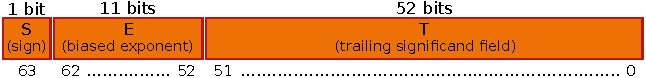
\includegraphics[width=0.7\linewidth]{\currentDir/floatIEEEStructure}%
\caption{The structure of an 64~bit / double precision IEEE~Standard 754 floating point number~\cite{IEEE2019ISFFPA,H1997IS7FPN}.}%
\label{fig:floatIEEEStructure}%
\end{figure}%
%
But how does it work in \python?
How can we deal with the fact that we cannot dynamically represent fractional numbers exactly even in typical everyday cases?
With \pythonil{float}, \python\ offers us one type for fractional numbers.
This datatype represents numbers usually in the same format as \pythonil{double}s in the \pgls{C}~programming language~\cite{PSF2024NTIFC}, which, in turn, internally have a 64~bit IEEE~Standard 754 floating point number layout~\cite{IEEE2019ISFFPA,H1997IS7FPN}.
The idea behind this standard is to represent both very large numbers, like~$10^{300}$ and very small numbers, like~$10^{-300}$.
In order to achieve this, the 64~bits are divided into three pieces, as illustrated in \cref{fig:floatIEEEStructure}.

The first part, the so-called \pgls{significand} or \pgls{mantissa}, consists of 52~bits, represents the digits of the number.
52~bits can represent $52\log_2 10\approx 15$~decimal digits, meaning that we can represent numbers to a precision of about 15~digits.
If we would just use 52~bits, then this would limit us to represent numbers maybe from~$0$ to~$2^{52}-1$ at a resolution of~$1$.
Of course, we could also choose some other resolution, say~$0.001$.
In this case, we could represent numbers from~$0$ to $0.001*(2^{52}-1)$ and the smallest non-zero number would be~$0.001$ instead of~$1$.
Whatever fixed resolution we would choose, it would be good in some cases and bad in others.

Therefore, the second part of the 64~bit floating point number representation comes into play:
The 11~bits of the \pgls{exponent} represent a power of~2 which is multiplied to the \pgls{significand} to get the actual number.
In order to allow us to have both small and large numbers, this value must be able represent positive and negative exponents.
Therefore, the stored value of the \pgls{exponent} is taken and a \pgls{bias} of~1023 is subtracted.
Thus, a stored value of 2000 in the exponent fields leads to an actual exponent of $1050-1023=27$, which would mean that the \pgls{significand} is multiplied with~$2^{27}$, i.e., $134\decSep217\decSep728$.%
%
\begin{sloppypar}%
Finally, the \pgls{signBit} in the floating point number dataformat indicates whether the number is positive or negative.
Together, this allows us to represent numbers from $2.225\decSep073\decSep858\decSep507\decSep201\decSep4*10^{-308}$ to $1.797\decSep693\decSep134\decSep8623\decSep157*10^{308}$ with a resolution of approximately 15~digits.
Of course, the same range also applies to negative numbers and $0$~can be represented as well.
Indeed, there are even special floating point values for infinity and errors.
But more about this later.%
\end{sloppypar}%
%
Luckily, you will never really need to know these exact information.
The important thing to remember is:
Floating point numbers can represent a wide range of different values.
Their range is large but still limited.
They can represent integers and fractions.
However, their accuracy is always limited to about 15~digits.
In other words, regardless whether your \pythonil{float} stores a very large or a very small number, you can have at most 15~digits of precision.
For example, adding~1 to~$10^{16}$ would still yield~$10^{16}$, because only 15~digits are \inQuotes{stored} and the~1 will just \inQuotes{fall off.}
You cannot represent numbers arbitrarily precisely.%
\endhsection%
%
\hsection{Floating Point Arithmetic}%
%
\begin{figure}%
\centering%
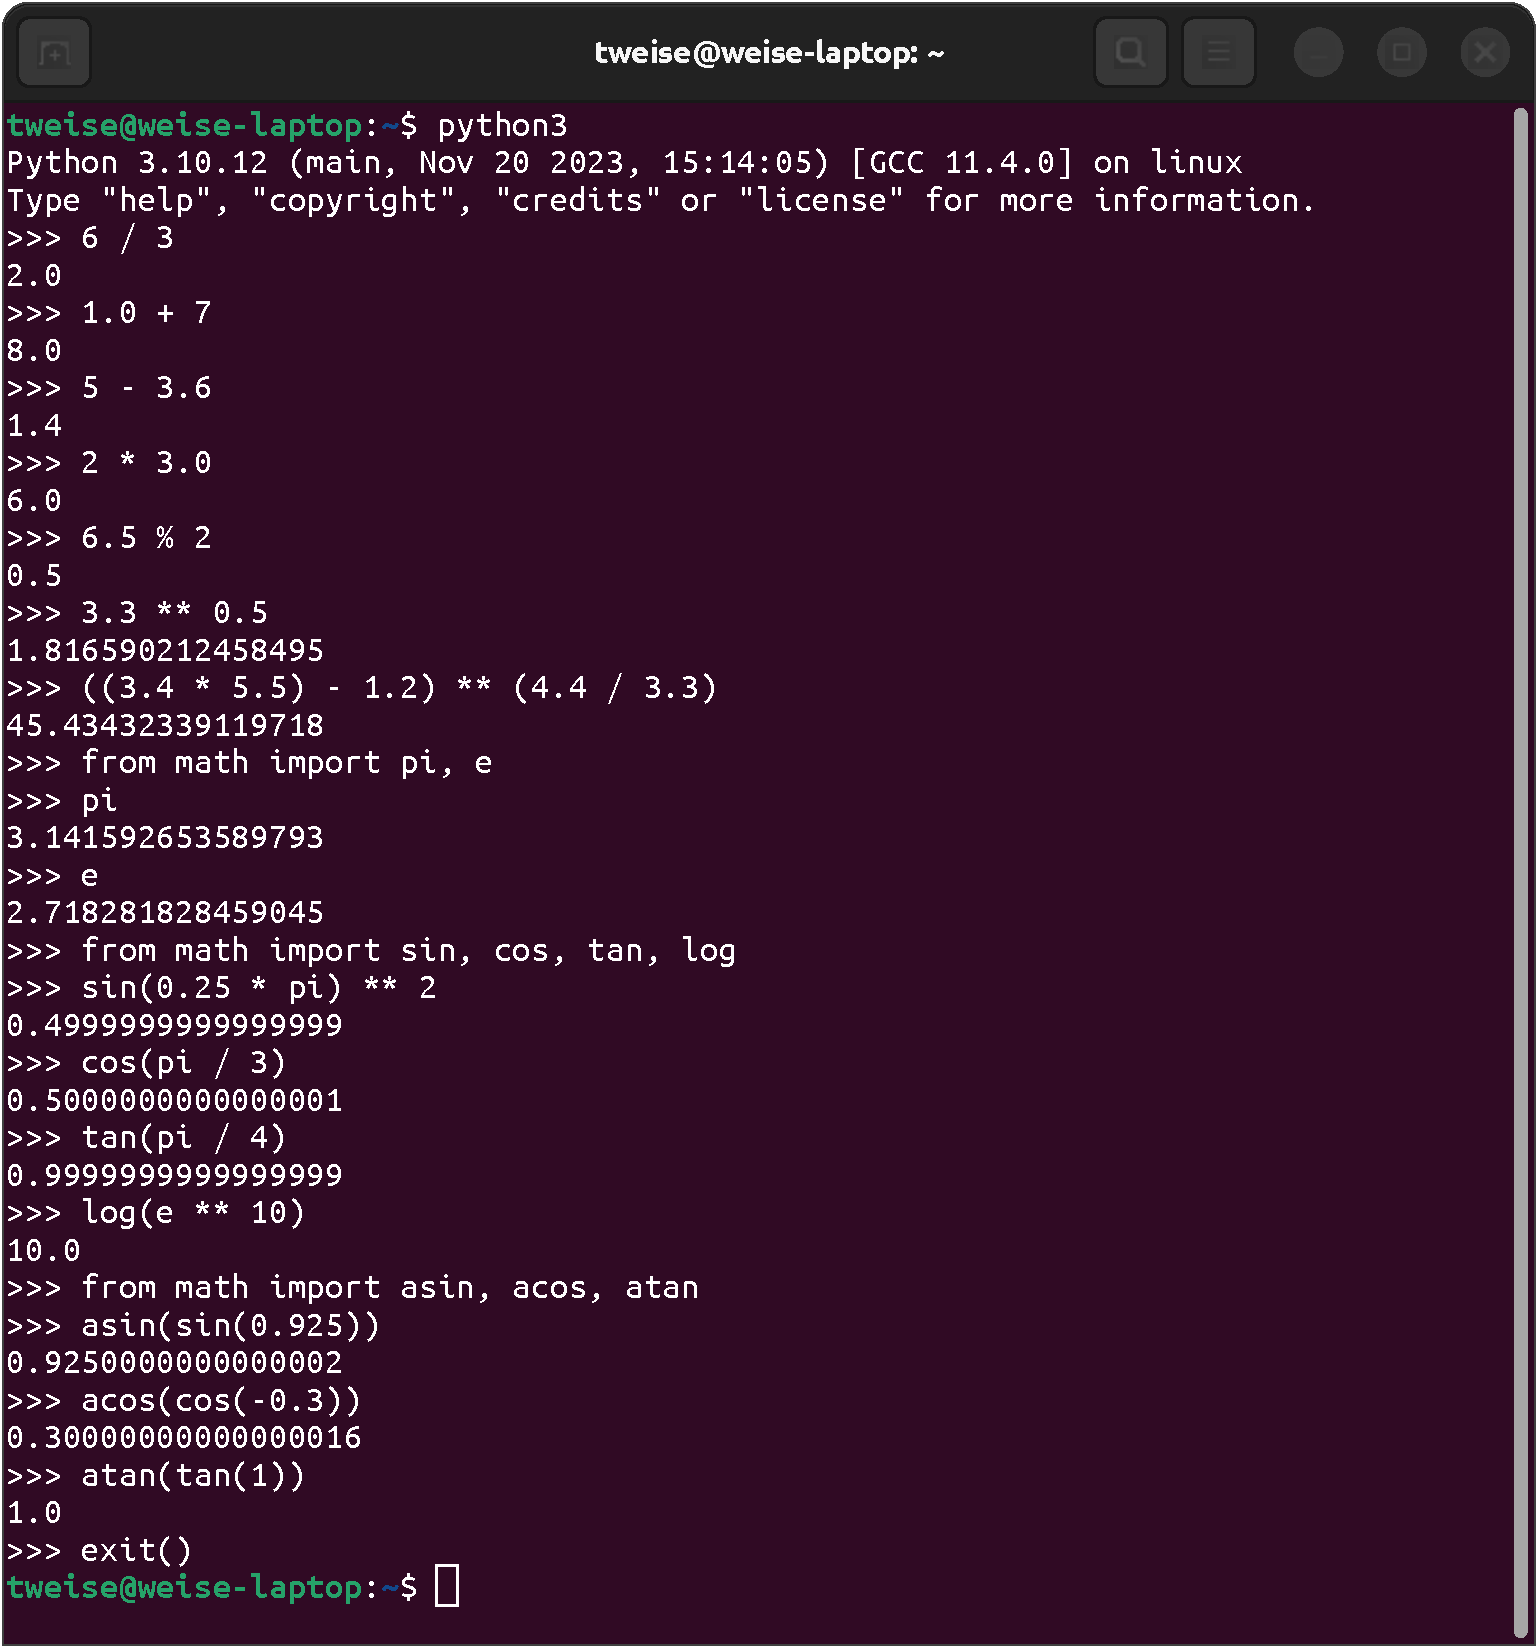
\includegraphics[width=0.8\linewidth]{\currentDir/floatMathInConsoleArith}%
\caption{Basic arithmetics with floating point numbers in \python.}%
\label{fig:floatMathInConsoleArith}%
\end{figure}%
%
Floating point numbers in \python\ can be distinguished from \pythonil{ints} by having a decimal dot in their text representation, i.e., \pythonil{5.0} is a \pythonil{float} and \pythonil{5} is an \pythonil{int}.
Let us now look at some examples for the basic arithmetic operations available for \pythonil{float}s in \cref{fig:floatMathInConsoleArith}.

We already learned that the division operator~\pythonil{/} always yields a \pythonil{float} result.
Therefore \pythonil{6 / 3} yields \pythonil{2.0} instead of \pythonil{2}.

The normal arithmetic operations like addition, subtraction, multiplication, division, and powers all work with \pythonil{float}s as expected.
Remember, however, that if \pythonil{float} and \pythonil{int} numbers are mixed, the results are always \pythonil{float}s.
Thus, \pythonil{1.0 + 7} gives us \pythonil{8} and \pythonil{2 * 3.0} yields \pythonil{6.0}.
In other words, if one \pythonil{float} occurs somewhere in an expression, it will \inQuotes{infect} everything that it touches to become a \pythonil{float} too, even if the result could be repreented as \pythonil{int}.
Some results cannot be integers anyway, for example \pythonil{5 - 3.6} evaluates to~\pythonil{1.4}.
The remainder (the modulo) of a division can also be computed for floating point numbers.
The remainder of the division of 6.5 by 2, i.e., \expandafter\pythonil{6.5 \% 2} is \pythonil{0.5}.

The square root of 3.3 can be computed as $3.3^{0.5}$.
\pythonil{3.3 ** 0.5} yields \pythonil{1.816590212458495}.
This brings us back to the previous section:
$\sqrt{3.3}$~is not actually 1.816\decSep590\decSep212\decSep458\decSep495.
It is an irrational number~\cite{S1988WPCHD,B1991IWNT} and irrational numbers cannot be expressed as fractions of integer numbers (by definition, otherwise they would be rational numbers).
Since they cannot be expressed as integer numbers, we cannot write them in any way like $\frac{1\decSep816\decSep590\decSep212\decSep458\decSep495\dots}{1\decSep000\decSep000\decSep000\decSep000\decSep000\dots}$, regardless of how large a denominator we would pick.
Hence, we cannot represent them exactly using discrete binary values of our computer's memory.
Hence, the floating point representation cuts off somewhere.
And this somewhere is after 15~decimal places.%
%
\begin{sloppypar}%
We can of course also write and compute more complex mathematical expressions.
\pythonil{((3.4 * 5.5) - 1.2) ** (4.4 / 3.3)} corresponds to $((3.4*5.5)-1.2)^{\frac{4.4}{3.3}}$ and yields \pythonil{45.43432339119718}.
This is again not an exact value but a rounded value.
We always need to keep this in mind.%
\end{sloppypar}%
%
Let us recall our initial example of the transcendental irrational numbers~$\pi$ and~$e$.
Certainly, these are very important constants that would be used in many computations.
We can make them accessible in our code by importing them from the \pythonil{math} module.\footnote{%
We will learn about these mechanism in detail later on.}
This can be done by typing \pythonil{from math import pi, e}.
When we then type \pythonil{pi} and \pythonil{e}, we can get to see their value in floating point representations: \pythonil{3.141592653589793} and \pythonil{2.718281828459045}, respectively.
Again, these are not the exact values, but they are as close as we can get in this format.

Of course, $\pi$ and~$e$ alone are not that much useful.
If you reach back into your highschool days again, you will remember many interesting functions that are related to them.
Let us import a few of them, again from the \pythonil{math} module, via \pythonil{from math import sin, cos, tan, log}.
I think you can guess what these functions do.

From highschool, you may remember that~$\sin{\frac{\pi}{4}}=\frac{\sqrt{2}}{2}$ and thus~$\sin^2{\frac{\pi}{4}}=0.5$.
Let us compute this in \python\ by doing \pythonil{sin(0.25 * pi) ** 2}.
Surprisingly, we get \pythonil{0.4999999999999999} instead of \pythonil{0.5}.
The reason is again the limited precision of \pythonil{float}, which cannot represent~$\frac{\sqrt{2}}{2}$ exactly.
Similarly, $\cos{\frac{\pi}{3}}=\frac{1}{2}$ but \pythonil{cos(pi / 3)} yields \pythonil{0.5000000000000001} and $\tan{\frac{\pi}{4}}$ expressed as \pythonil{tan(pi / 4)} returns \pythonil{0.9999999999999999} instead of~$1$.
Then again, these values are incredibly close to the exact results.
They are off by \emph{less than~$10^{-15}$} so for all practical concerns, they are close enough.
Sometimes, we even get the accurate result, e.g., when computing $\ln(e^{10})$ by evaluating \pythonil{log(e ** 10)}, which results in~\pythonil{10.0}.

As final example for floating point arithmetics, let us import the inverse trigonometric functions by doing \pythonil{from math import asin, acos, atan}.
Obviously, $\arcsin{\sin{0.925}}$ should be~$0.925$.
Calculating \pythonil{asin(sin(0.925))} indeed yields~\pythonil{0.9250000000000002}.
Due to the periodicity of the trigonometric functions, $\arccos{\cos{-0.3}}$ is~$0.3$ and \pythonil{acos(cos(-0.3))} results in~\pythonil{0.30000000000000016}.
For $\arctan{\tan{1}}$ we even get the exact result \pythonil{1.0} by computing \pythonil{atan(tan(1))}.%
%
\endhsection%
%
\endhsection%
%
